\section{Implementation Outline}
The goal is to translate the raw data from the cameras into an image format that is compatible with the \gls{h265} encoder, specifically the \gls{p010} format.
The \gls{p010} format is a YCbCr 4:2:0 format with interlaced chroma data.
In this format, each channel is represented by 10 bits per pixel stored in the most significant bits of 16-bit little-endian unsigned integers.

This conversion can be divided into five parts: unpacking the raw bits from the camera, separating different polarization angles, performing debayering, converting to YCbCr color space, applying chroma subsampling, and finally, arranging the data in the correct format.
The entire process is visualized in Figure \ref{fig:transform}.
This approach is inspired by the work of Vy Nguyen et al., where they perfom the color demosaicing on the polarization channels separately \cite{nguyenTwoStepColorPolarizationDemosaicking2022}.


\begin{figure}[H]
    \centering
    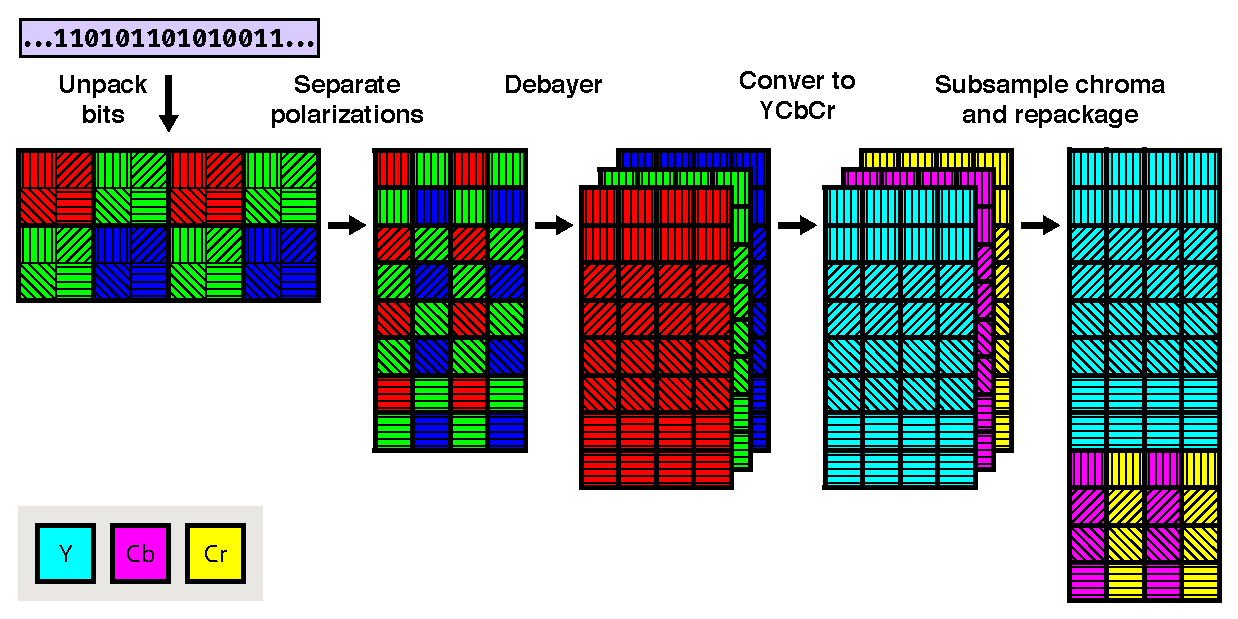
\includegraphics[width=\textwidth]{figures/polarized_image/transform.pdf}
    \caption{Visualization of how raw data is transformed into a YCbCr format where the angles of polarization are stacked vertically.}
    \label{fig:transform}
\end{figure}


Initially, I attempted to perform these steps using \gls{numpy} for data unpacking and \gls{opencv} for the transformations.
However, even when utilizing all eight \gls{cpu} cores on the \jx to their full extent, I was unable to achieve the required performance.
Furthermore, running the \gls{cpu} cores at maximum frequency had a substantial negative impact on the power consumption of the \jx.

To attain the necessary throughput, I made the decision to implement the whole translation process using\gls{cuda}.
This implementation is divided into two parts: data unpacking and transformation.
While\gls{cuda}-accelerated \gls{opencv} was considered, significant optimization potential was identified due to the unique format of the camera sensors.
